\documentclass[11pt,a4paper]{article}
\usepackage{fontspec}
\setmainfont{TeX Gyre Pagella}
\newfontfamily\headfont{Inter}[UprightFont=*-ExtraBold,BoldFont=*-ExtraBold,Extension=.otf,Path=/usr/share/fonts/opentype/inter/]
\usepackage[a4paper,margin=2.3cm]{geometry}
\usepackage{graphicx}
\graphicspath{ {../blog/} }
\usepackage{booktabs,float,caption,array,xcolor}
\usepackage[hidelinks]{hyperref}
\usepackage{titlesec}
\usepackage{setspace}
\usepackage[round]{natbib}
\setstretch{1.05}
\renewcommand{\topfraction}{0.9}
\renewcommand{\bottomfraction}{0.8}
\renewcommand{\textfraction}{0.1}
\renewcommand{\floatpagefraction}{0.75}
\setlength{\parindent}{0pt}
\setlength{\parskip}{0.55em}
\titleformat{\section}{\headfont\Large}{\thesection}{0.8em}{}
\titleformat{\subsection}{\headfont\large}{\thesubsection}{0.8em}{}
\captionsetup{font=small,labelfont=bf}
\urlstyle{same}
\hypersetup{pdftitle={How High Is the World?},pdfauthor={Tristan Hotham}}

\begin{document}
\begin{center}
{\Large\bfseries How High Is the World?\\[2pt] Height Above Sea Level, Mountains and Where People Live, from Open Terrain Data\par}
\vspace{1.2em}
{\large Tristan Hotham\par}
\vspace{0.3em}
{\small Independent researcher\\
ORCID: 0000-0003-4931-9349\\
DOI: \url{https://doi.org/10.5281/zenodo.23848930}\par}
\vspace{0.8em}
2026
\end{center}

\begin{quote}
\small
\begin{center}\textbf{Abstract}\end{center}
I describe the height of the world's land from the open AWS Terrain Tiles (Mapzen's Terrarium mosaic of SRTM, GMTED2010, ETOPO1 and national elevation models), using the zoom 4 level of the tiles as a 4,096 by 4,096 Web Mercator grid of about 9.8 km at the equator, with every cell weighted by its true area and land defined by Natural Earth countries less lakes. The world's land averages 807 m above sea level (678 m without Antarctica) with a median of 432 m; 26\% of it lies above 1,000 m, 11\% above 2,000 m and 0.5\% above 5,000 m. Antarctica is the highest continent (2,208 m) and Asia the highest without ice (1,059 m); among countries large enough to be resolved, Tajikistan (2,961 m) is the highest and the Netherlands (10 m) the lowest. About 355,893 km² of land in named depressions lies below sea level at this resolution, 76\% of it around the Caspian. I check 136,410 Wikidata peaks against the terrain, keeping 134,657, and confirm the highest point of 189 countries against an independent list. Finally, of the 2.6 billion people in 4,325 Wikidata cities of 50,000 or more, 10.3\% live above 1,000 m and 1.9\% above 2,000 m: people live far lower than the land lies. An interactive map draws the same tiles at every zoom with a height readout for any point.

\textbf{Keywords:} elevation; hypsometry; topography; mountains; prominence; height above sea level; cities; SRTM; Wikidata; open data; mapping
\end{quote}

\section{Introduction}
Height above sea level is one of the first facts we learn about a place and one of the least often mapped well. It sets climate, vegetation and the cost of moving and building, and it has long been summarised by the hypsometric curve: the share of a region's area that lies above each height \citep{strahler}. Global elevation models now make it possible to draw that curve, and the map behind it, for the whole planet from open data. The most convenient form is the set of web tiles first built by Mapzen and now hosted as an open dataset by Amazon \citep{terraintiles}, which merge the Shuttle Radar Topography Mission \citep{srtm}, GMTED2010 \citep{gmted}, ETOPO1 \citep{etopo1} and many national models into one global mosaic at every web map zoom level.

This study does three things. It measures the height of the world's land, by continent and by country, from the coarsest level of those tiles, weighting every cell by its true area and stating plainly what a 10 km grid can and cannot resolve. It assembles and checks open data on peaks and on the height of cities, which are messier than they look. And it builds an interactive map (\url{https://maps.tristanhotham.com/world-terrain/}) that decodes the tiles in the browser at every zoom, with height tints, shaded relief, height steps and a readout of the height of any point.

\section{Data}
\textbf{Terrain.} The AWS Terrain Tiles in Terrarium encoding are 256 pixel PNG tiles in Web Mercator in which each pixel's colour encodes a height: height = R $\times$ 256 + G + B / 256 $-$ 32,768 metres. Land heights come from SRTM (3 arc seconds, about 90 m, and 1 arc second in the United States), national models (for example NED and 3DEP in the United States, the Canadian Digital Elevation Data, EU-DEM, Geoscience Australia's and LINZ's models, INEGI's for Mexico and Ordnance Survey's OS Terrain 50 for Great Britain), GMTED2010 at coarser levels and outside SRTM's coverage, and ArcticDEM in the far north; sea floor heights come from ETOPO1 and other bathymetry \citep{joerd}. Heights are relative to mean sea level (for SRTM, the EGM96 geoid). I use the 256 tiles of zoom level 4, which form a 4,096 by 4,096 grid covering the world between 85.05 degrees north and south; a cell is 9.8 km across at the equator and 4.9 km at 60 degrees. For the part of Antarctica south of 85.05 degrees I use ETOPO10, a 10 arc minute grid derived from ETOPO1 (ice surface).

\textbf{Land.} Natural Earth's 1:10m countries \citep{naturalearth}, less its lakes and reservoirs (salt pans such as Kati Thanda-Lake Eyre stay land), define land and the country of each cell.

\textbf{Peaks.} Every Wikidata item that is a mountain, hill, summit or volcano of any kind with an elevation (P2044), as stated and as normalised to metres by Wikidata from the statement's unit, with prominence (P2660), coordinates, country and number of sitelinks: 161,049 rows for 136,410 distinct items \citep{wikidata}. I add the few summits Wikidata lacks or cannot place from Natural Earth's elevation points (public domain) and from the 125 most prominent summits in English Wikipedia's list of peaks by prominence \citep{wpprom}, which also supplies the prominence ranking; both carry Wikidata identifiers.

\textbf{Cities.} Wikidata items for cities of 50,000 or more people with an elevation and a population: 4,373 items.

\textbf{Check list.} A list of the highest point of each country compiled from peakbagger.com, used only to check the open data and not republished.

\begin{table}[tbp]\centering\small\caption{Sources, what was used and licences.}\label{tab:sources}\begin{tabular}{>{\raggedright\arraybackslash}p{3.6cm}>{\raggedright\arraybackslash}p{7.4cm}>{\raggedright\arraybackslash}p{3.4cm}}\toprule Source & Used & Licence\\\midrule
AWS Terrain Tiles (Terrarium) & Zoom 4 grid for statistics; all zooms on the map & Per source; mostly public domain, some CC BY or OGL\\
ETOPO10 (from ETOPO1) & Antarctica south of 85.05 S; polar caps for the Earth curve & Public domain\\
Wikidata & 136,410 peak items, 4,373 city items & CC0\\
Natural Earth & Countries, lakes, places; 89 added summits & Public domain\\
English Wikipedia & 125 most prominent summits (3 added) & CC BY-SA 4.0\\
peakbagger.com list & National high points, check only & Not redistributed\\
\bottomrule\end{tabular}\end{table}

\section{Methods}
\subsection{The grid and its statistics}
The 256 tiles are mosaicked and decoded to heights. 13 cells differ from the median of their eight neighbours by more than 2,500 m in a way no real terrain does (a spike of 11,500 m on Baffin Island, holes several kilometres deep in shallow ground); they are replaced by that median. Small islands a few metres high amid deep ocean, which look similar, are kept.

Each cell's true area is computed exactly from its two bounding latitudes on a sphere of radius 6,371 km. Natural Earth countries and lakes are rasterised on a grid twice as fine, so every cell carries the share of its area that is land and the share that belongs to each country. A coastal cell's height averages land with sea floor, so for land statistics I floor heights at 0 m except in cells that are wholly land and surrounded by wholly-land cells; only those interior cells may be below sea level. Ice counts at its surface. Shares, medians and the hypsometric curve come from area-weighted histograms in 5 m bins (25 m for countries); means are exact area-weighted means. A country is treated as resolved, and ranked, if it covers at least 100 cells.

\subsection{Peaks}
Rows are merged by Wikidata item, and the metre value normalised from the preferred statement is tried first. Each candidate height is compared with the 5 by 5 block of cells around the point (about 50 km at the equator): a summit can rise well above the highest 10 km average nearby, but across 15,000 European summits the excess over that highest cell, measured in units of the local relief plus 300 m, stays below 0.8 for 99.9\% of them, and for Natural Earth's 630 named mountains below 1.22 for 95\%, with the largest values on small islands. A height that is implausible in metres but plausible in feet (excess above 3.0 away from small islands, or higher than every summit of its continent in Natural Earth), which points to a unit entered wrongly, is converted; values below 10 that only fit as kilometres are converted; heights that fit nothing are dropped. Natural Earth's or Wikipedia's height is used only when no Wikidata value fits. Finally, a summit away from the coast that is more than 30 m higher than the independent high point of every country it lies in is dropped. A summit's countries are the Natural Earth countries within 1 km of its point, plus its Wikidata country if that lies within 25 km, plus the country named in the Wikipedia list.

\subsection{Cities}
Duplicate rows are merged (largest population; the height and point that best fit the grid), metropolitan areas, provinces, districts and similar aggregates are dropped, as is a second item of the same name within 10 km of a larger one. A city's height must lie between the lowest and highest cells of the 3 by 3 block around it, with allowances for relief; values that only fit in feet are converted for American and British items and others dropped. Wikidata gives Chinese prefecture-level cities the population of the whole prefecture, so in the ranking of cities of a million or more a Chinese city counts only if Natural Earth's populated places give the same place, within 30 km, an urban population of a million or more, and that figure is shown; 84 are left out, among them Lijiang (2,400 m) and Zhaotong.

\section{Results}
\subsection{The hypsometry of the land}
The world's land, 145.6 million km² including Antarctica's ice and excluding lakes, has a mean height of 807 m and a median of 432 m (Figure~\ref{fig:hyps}). 45\% lies above 500 m, 26\% above 1,000 m, 11\% above 2,000 m, 5.1\% above 3,000 m, 1.8\% above 4,000 m and 0.5\% above 5,000 m. Antarctica, 12.2 million km² at a mean of 2,208 m, dominates the upper middle of the curve: without it the land averages 678 m, with 21\% above 1,000 m and 6.5\% above 2,000 m; without Greenland's ice too, 660 m. The mean is a little below the figure of about 840 m often quoted for the land, as expected for a smoothed grid whose coastal cells are floored at sea level.

Over the whole Earth, land and sea floor together, 29.6\% of the surface lies above sea level and the sea floor averages 3,713 m down (a second curve on the interactive page).

\begin{figure}[tbp]\centering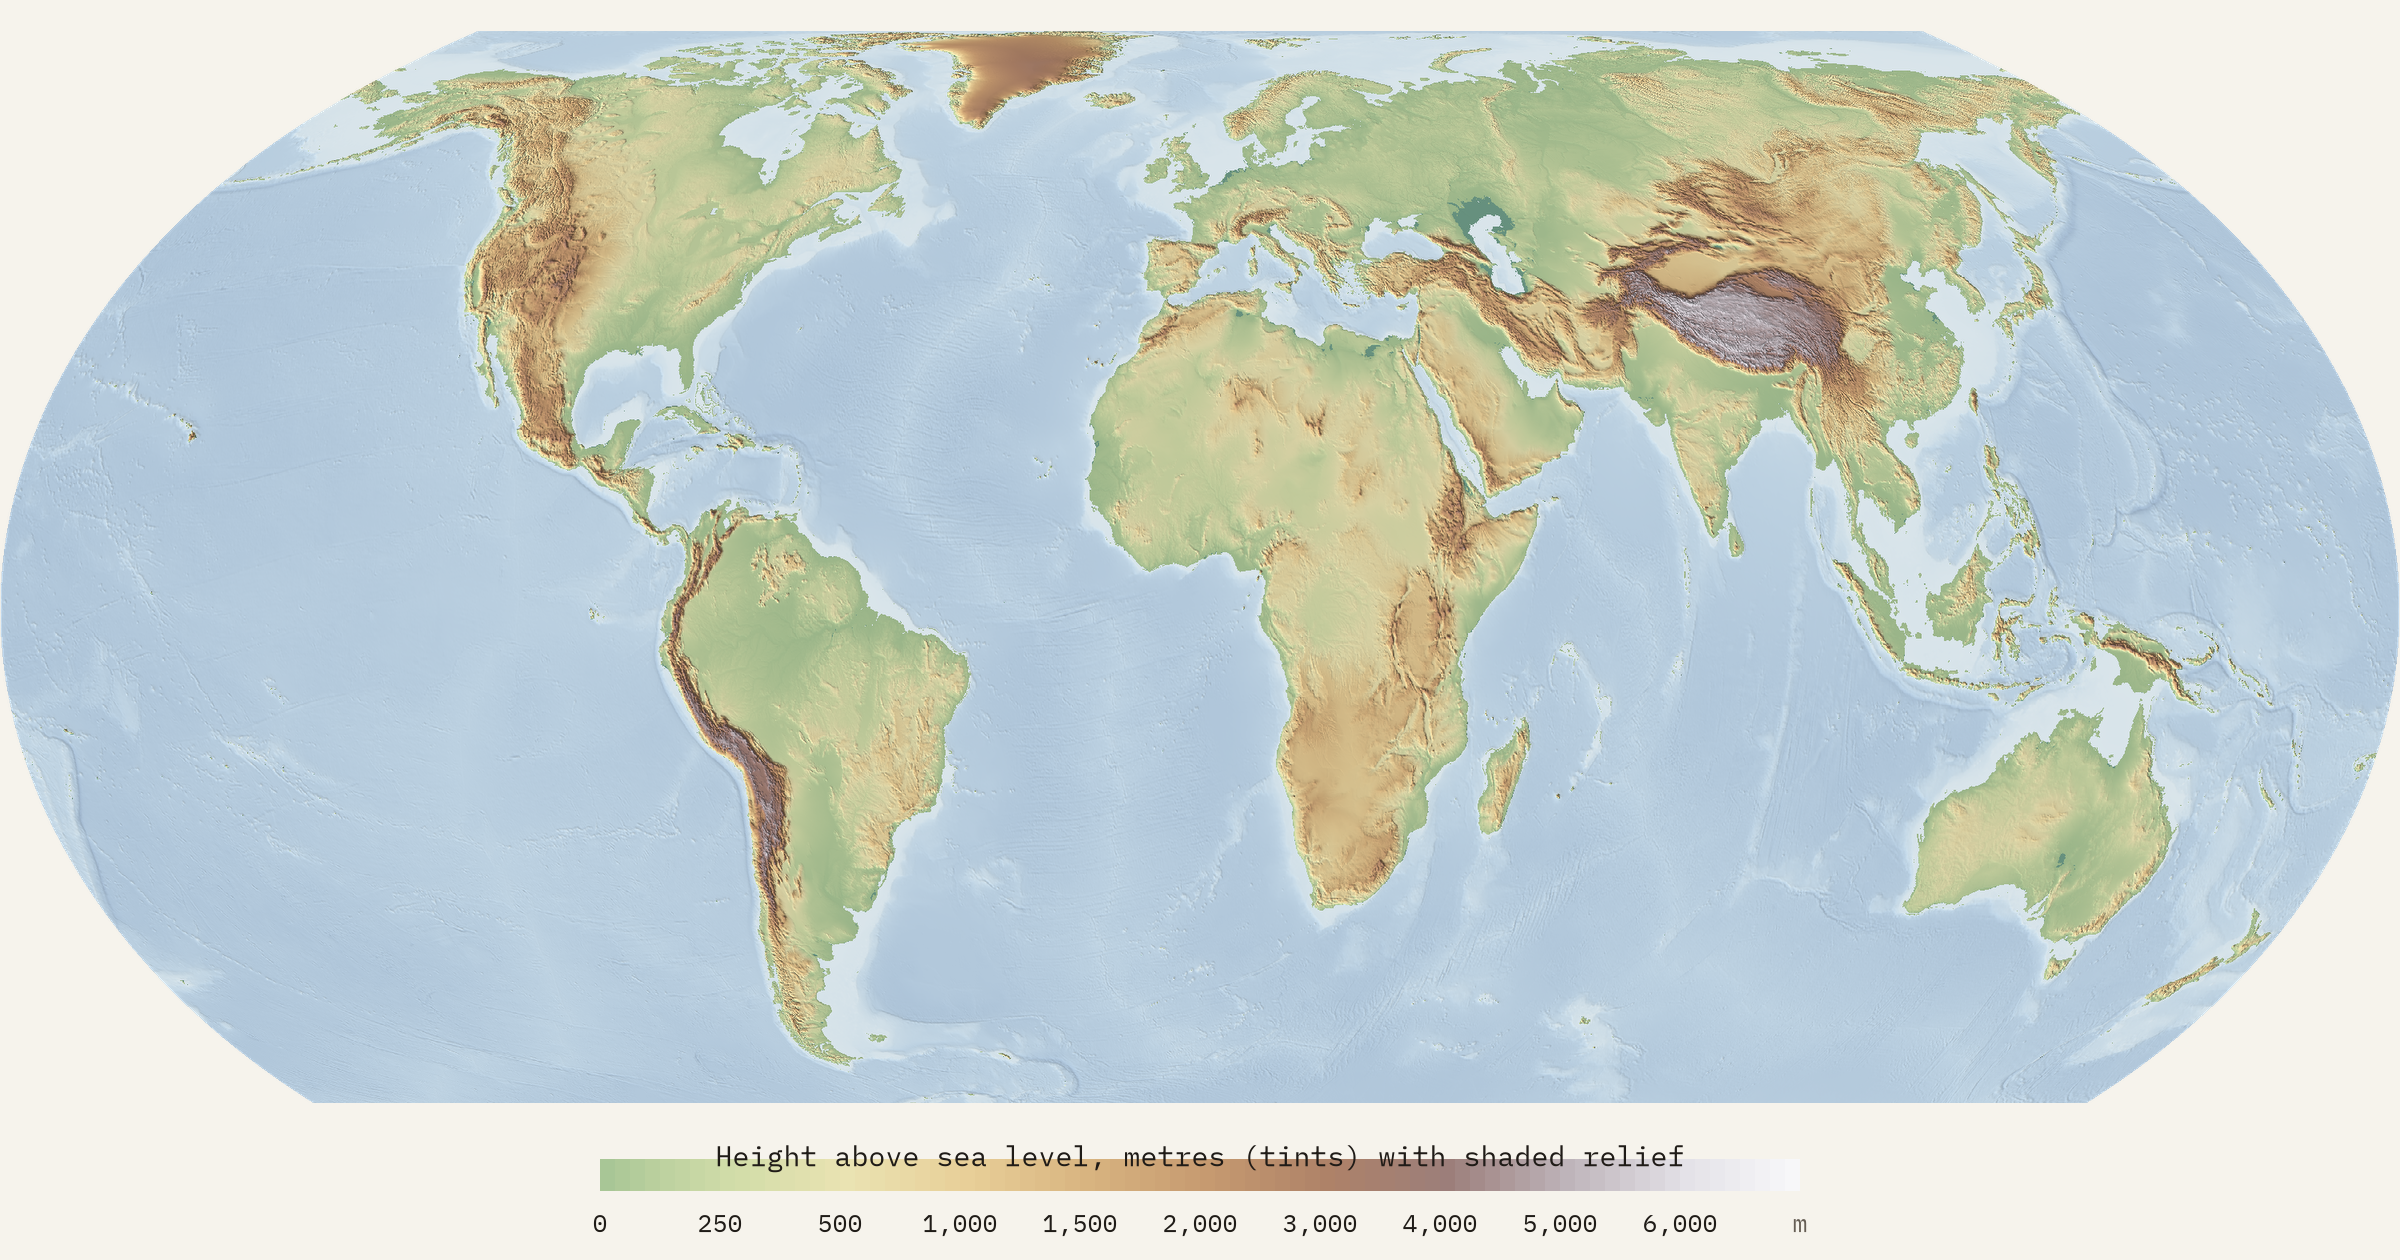
\includegraphics[width=\linewidth]{b_world_relief.png}\caption{Height above sea level, with shaded relief (vertical exaggeration 24 times), from the zoom 4 AWS Terrain Tiles resampled to 0.075 degrees and shown in the Equal Earth projection.}\label{fig:map}\end{figure}
\begin{figure}[tbp]\centering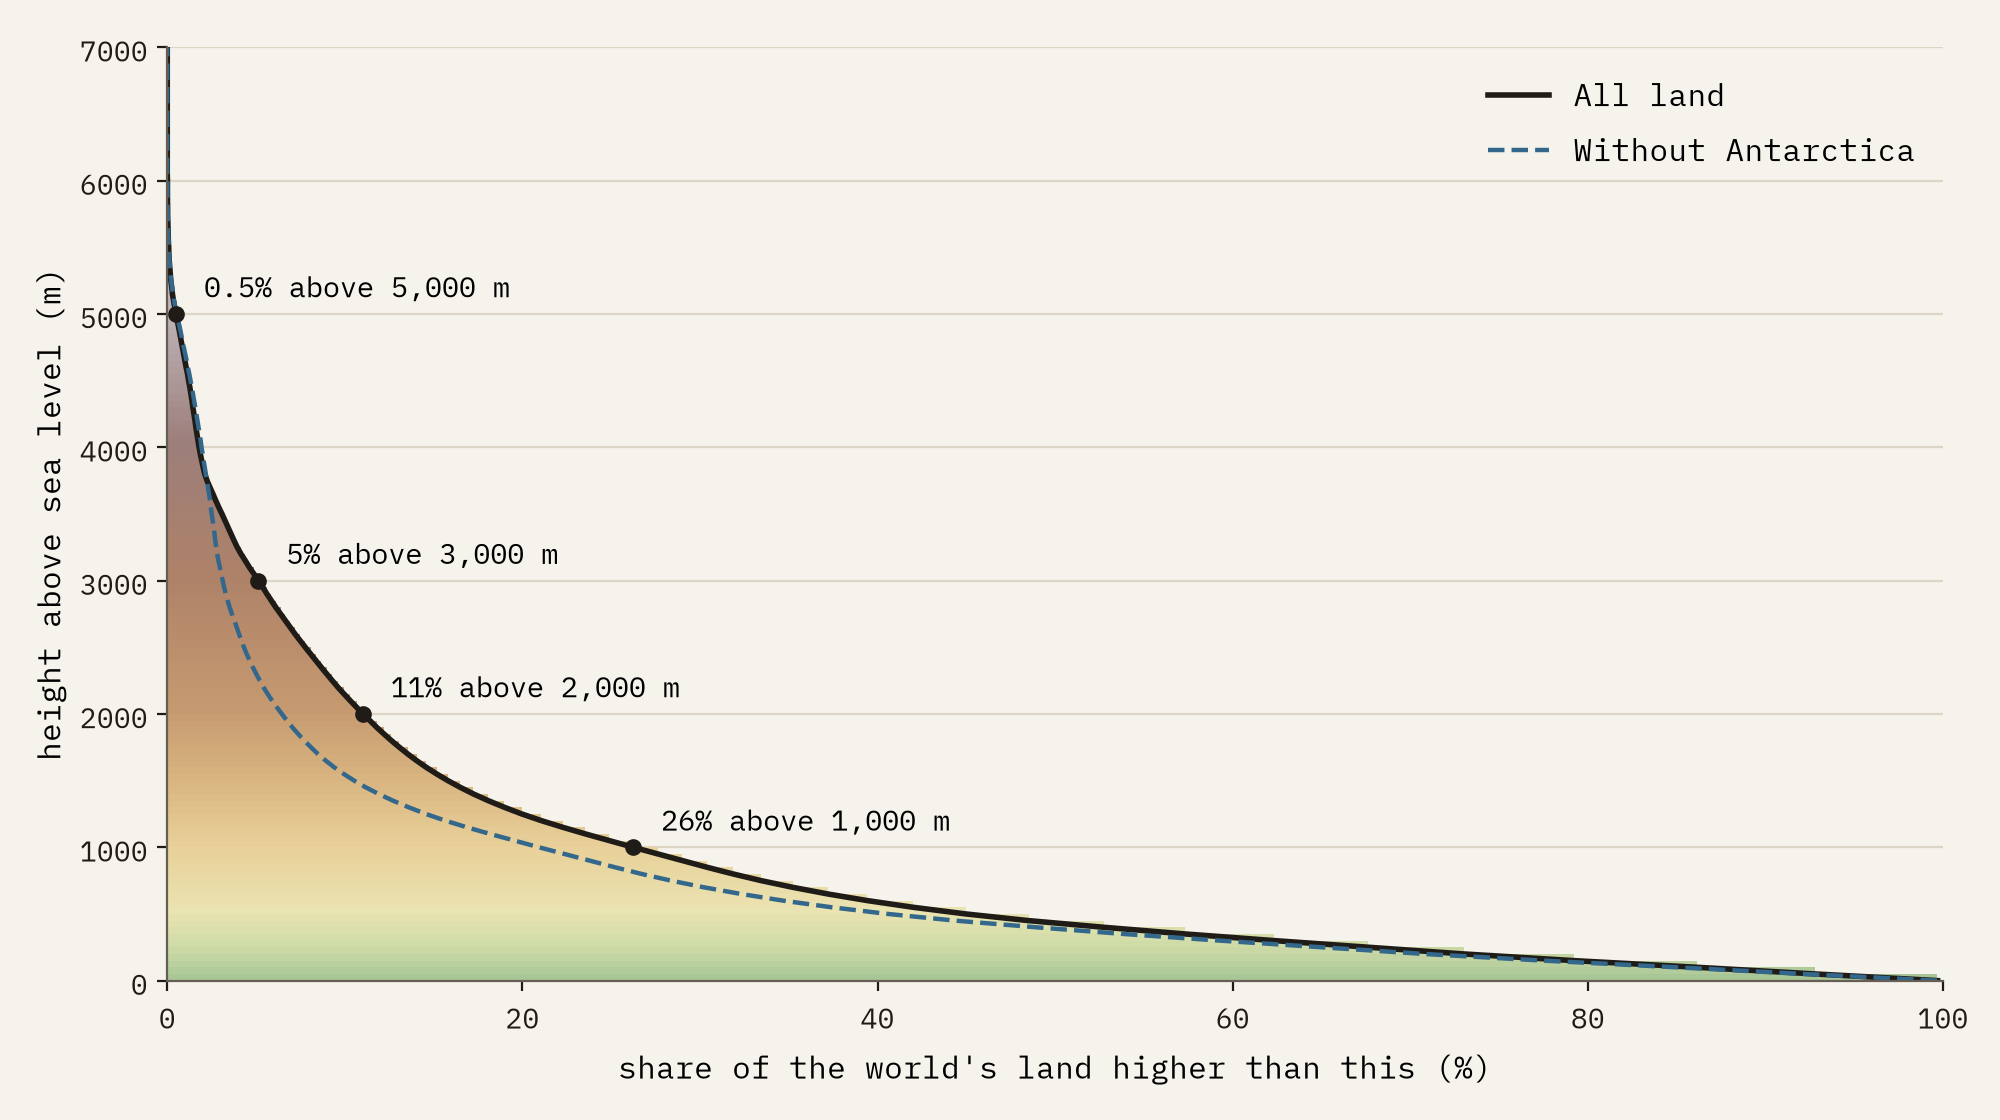
\includegraphics[width=.86\linewidth]{b_hypsometry.png}\caption{Hypsometric curve of the world's land: share of land area higher than each height, with and without Antarctica.}\label{fig:hyps}\end{figure}

\subsection{Continents and countries}
By Natural Earth's continents, Antarctica is highest (2,208 m), then Asia (1,059 m), North America (740 m, raised by Greenland's ice), Africa (629 m), South America (587 m), Europe (370 m) and Oceania (301 m) (Figure~\ref{fig:countries}). Among the 161 countries covering at least 100 cells, the highest on average are Tajikistan (2,961 m), Bhutan (2,763 m), Kyrgyzstan (2,683 m), Lesotho (2,218 m) and Nepal (2,013 m); the lowest are the Netherlands (10 m), Bahamas (24 m), The Gambia (24 m), Qatar (27 m) and Bangladesh (28 m). Lesotho and Rwanda are the only countries in the ranking whose lowest cell lies above 1,000 m (Lesotho's is at 1,454 m). Table~\ref{tab:countries} gives more.

The grid smooths these values. Nepal's mean of 2,013 m is lower than figures often quoted, because the deep valleys and high ridges of the Himalaya are averaged together and the flat Terai is large; and the highest cell in the whole grid is 6,727 m, 2,122 m below the summit of Everest.

\begin{table}[tbp]\centering\small\caption{The ten highest and ten lowest countries by mean height of land (countries covering at least 100 cells of the zoom 4 grid). Median from 25 m bins; highest 10 km cell; share of land above 2,000 m (\%).}\label{tab:countries}\begin{tabular}{lrrrr}\toprule Country & Mean m & Median m & Highest cell m & Above 2,000 m\\\midrule
Tajikistan & 2,961 & 3,362 & 5,741 & 69\\
Bhutan & 2,763 & 2,762 & 6,343 & 66\\
Kyrgyzstan & 2,683 & 2,812 & 5,636 & 72\\
Lesotho & 2,218 & 2,212 & 3,196 & 64\\
Nepal & 2,013 & 1,488 & 6,494 & 40\\
Armenia & 1,853 & 1,888 & 3,357 & 42\\
China & 1,830 & 1,162 & 6,727 & 32\\
Afghanistan & 1,804 & 1,588 & 5,654 & 41\\
Greenland & 1,803 & 1,988 & 3,310 & 49\\
Rwanda & 1,694 & 1,612 & 2,934 & 16\\
\midrule
Netherlands & 10 & 12 & 209 & 0\\
Bahamas & 24 & 12 & 549 & 0\\
The Gambia & 24 & 12 & 57 & 0\\
Qatar & 27 & 38 & 69 & 0\\
Bangladesh & 28 & 12 & 646 & 0\\
Denmark & 30 & 38 & 126 & 0\\
Guinea-Bissau & 38 & 38 & 167 & 0\\
Senegal & 54 & 38 & 459 & 0\\
Estonia & 59 & 62 & 261 & 0\\
Latvia & 90 & 88 & 251 & 0\\
\bottomrule\end{tabular}\end{table}
\begin{figure}[tbp]\centering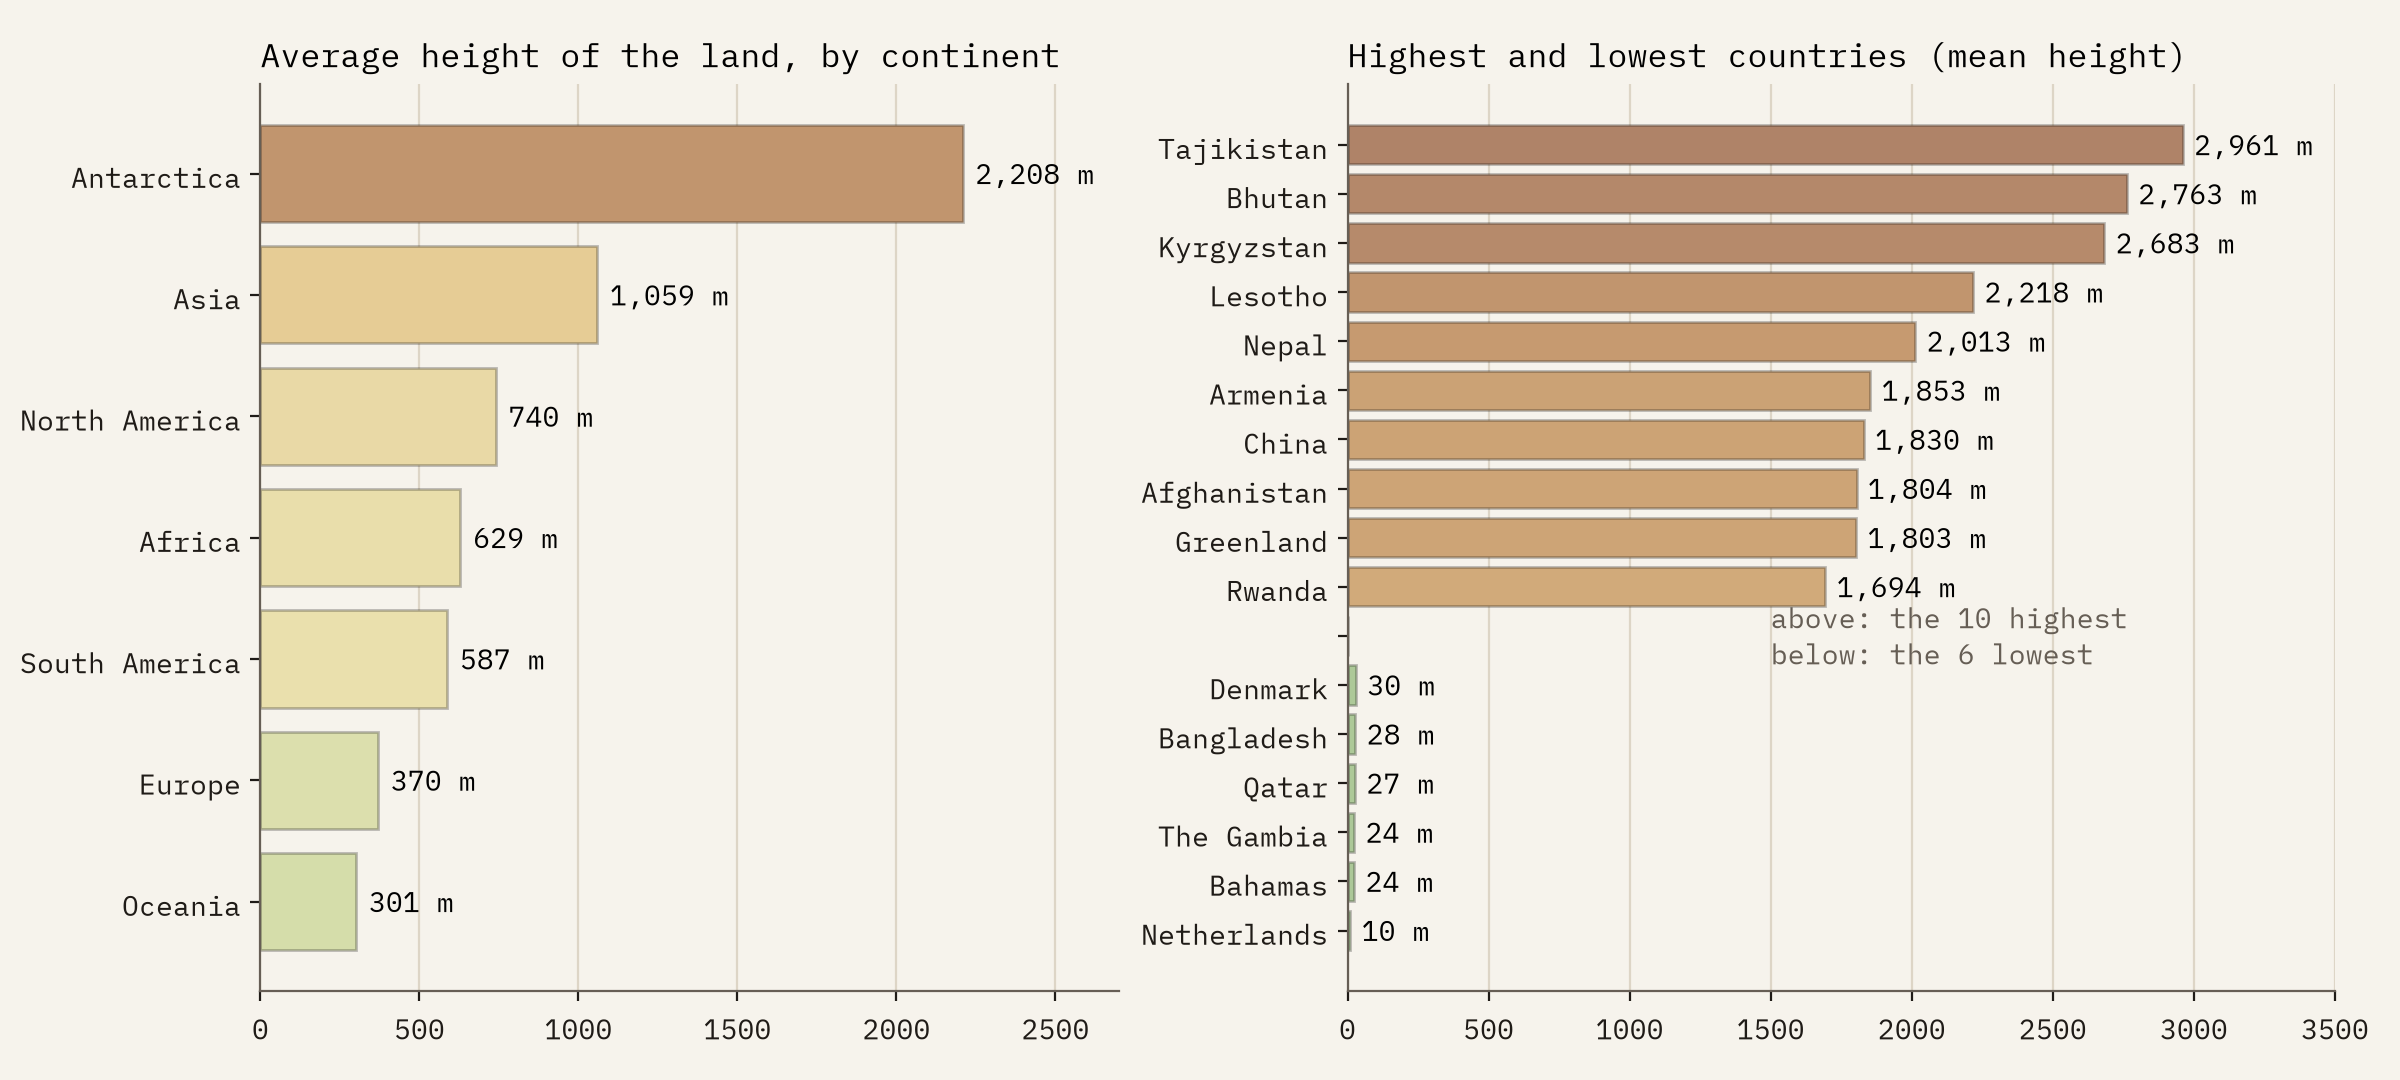
\includegraphics[width=\linewidth]{b_countries.png}\caption{Mean height of land by continent, and the highest and lowest countries among those covering at least 100 grid cells.}\label{fig:countries}\end{figure}

\subsection{Land below sea level}
Interior land cells below 0 m, outside Antarctica and Greenland, form 1,104 patches. Named depressions add up to 355,893 km²: the Caspian Depression (269,883 km²), Qattara (22,007 km²), Kati Thanda-Lake Eyre (13,474 km²), the Netherlands (11,300 km²), Afar and Danakil (8,920 km²), the Dead Sea and Jordan valley (4,514 km², lowest cell -478 m) and smaller basins down to Death Valley (680 km²) (Figure~\ref{fig:below}). A further 89,568 km² of small patches on deltas and coastal flats is partly real and partly sea floor averaged into coastal cells, and is not counted.
\begin{figure}[tbp]\centering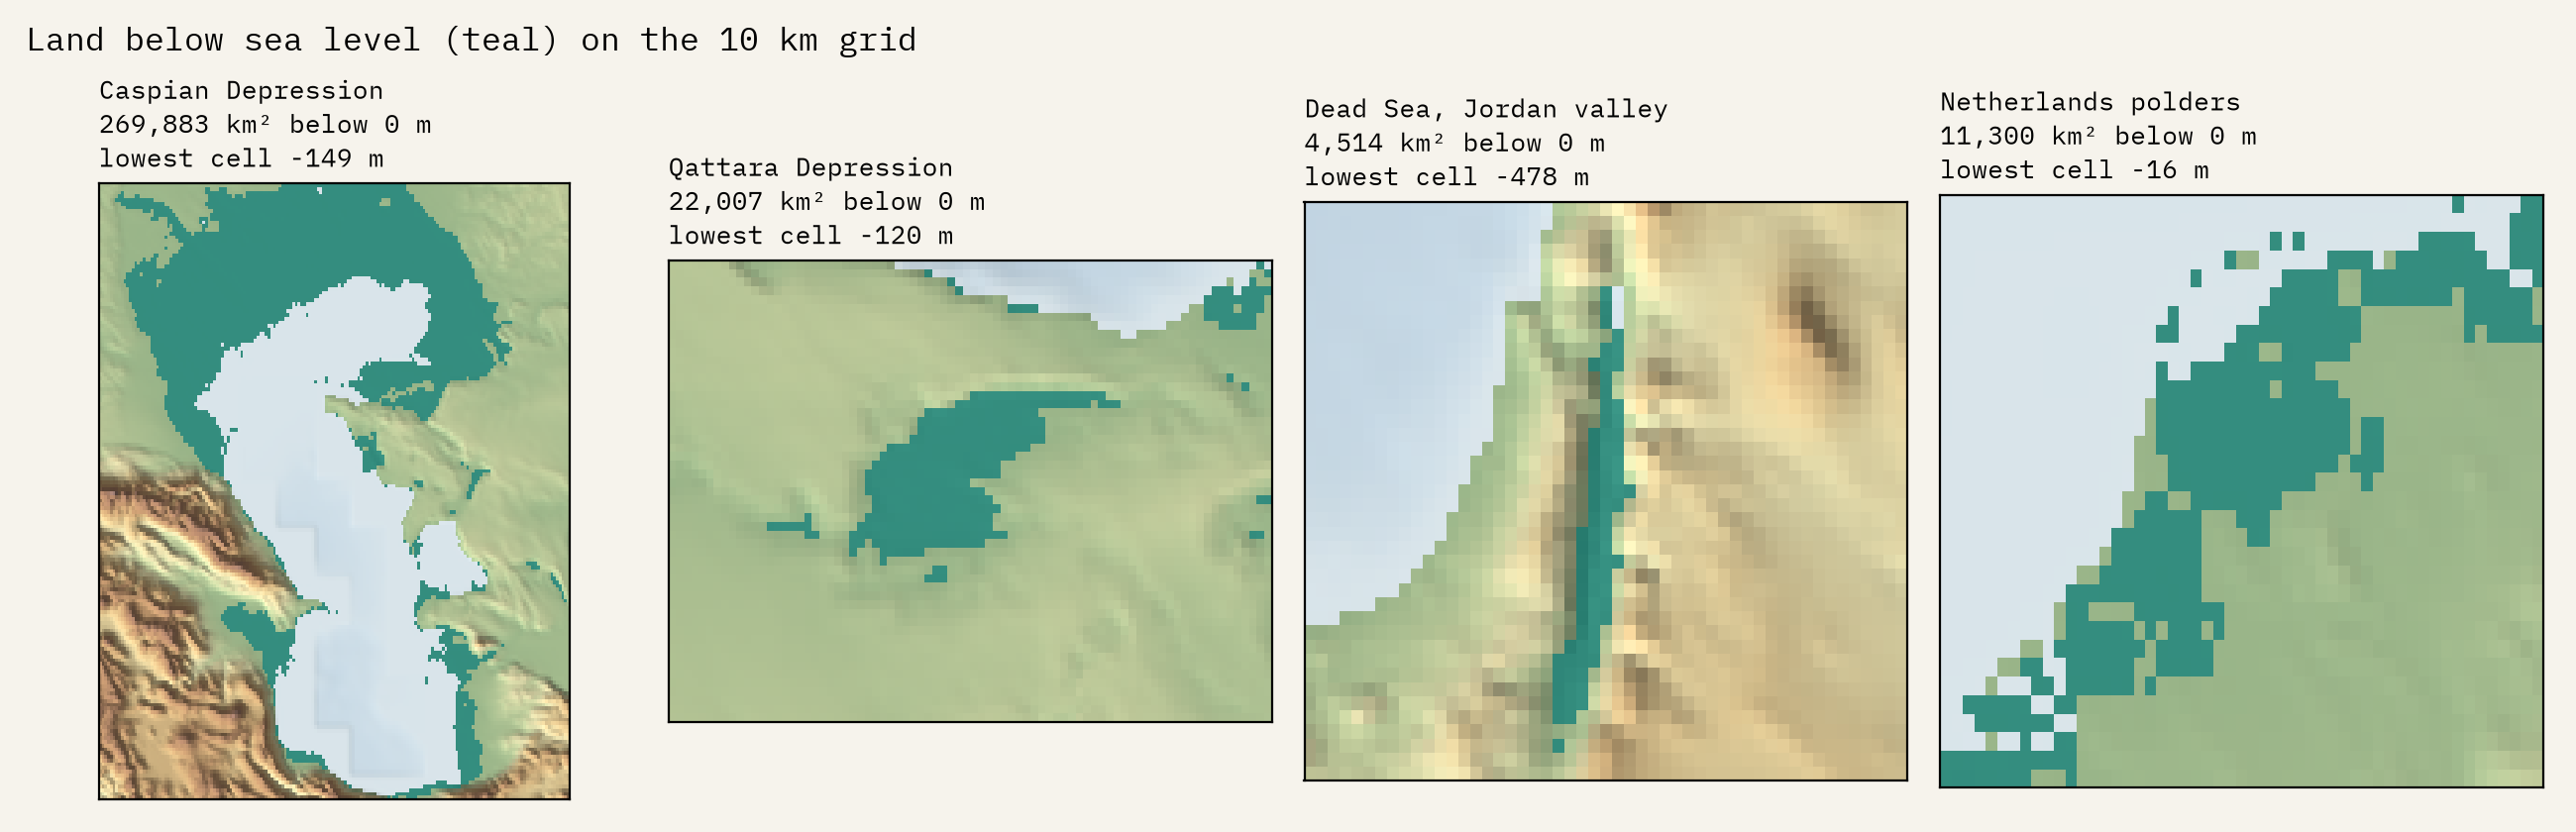
\includegraphics[width=\linewidth]{b_below_sea.png}\caption{Land below sea level (teal) on the 10 km grid in four depressions.}\label{fig:below}\end{figure}

\subsection{Peaks}
Cleaning left 134,657 summits. 3,057 heights were stated in feet in Wikidata and normalised; the checks converted a further 18 from feet and 15 from kilometres, and 1,845 items were dropped (1,383 of them for lack of coordinates). The highest summit of each continent is Everest (8,849 m), Aconcagua (6,962 m), Denali (6,190 m), Kilimanjaro (5,895 m), Elbrus (5,642 m), Vinson Massif (4,892 m) and, by Natural Earth's continents, Mount Wilhelm (4,509 m) in Papua New Guinea; Puncak Jaya (4,884 m) lies in Indonesia and so in Asia. By prominence (Figure~\ref{fig:prom}), Everest, Aconcagua (6,961 m), Denali (6,155 m) and Kilimanjaro (5,885 m) lead; K2 is 22nd.

The highest summit in the cleaned data agrees within 30 m with the independent list of national high points for 189 of the 215 countries in both. In 10 the open data lacks the true summit and in 6 it has no summit at all; in 10 it has a higher one, for reasons that include definitions (Mount Scenery on Saba is the highest point of the Kingdom of the Netherlands) as well as errors.
\begin{figure}[tbp]\centering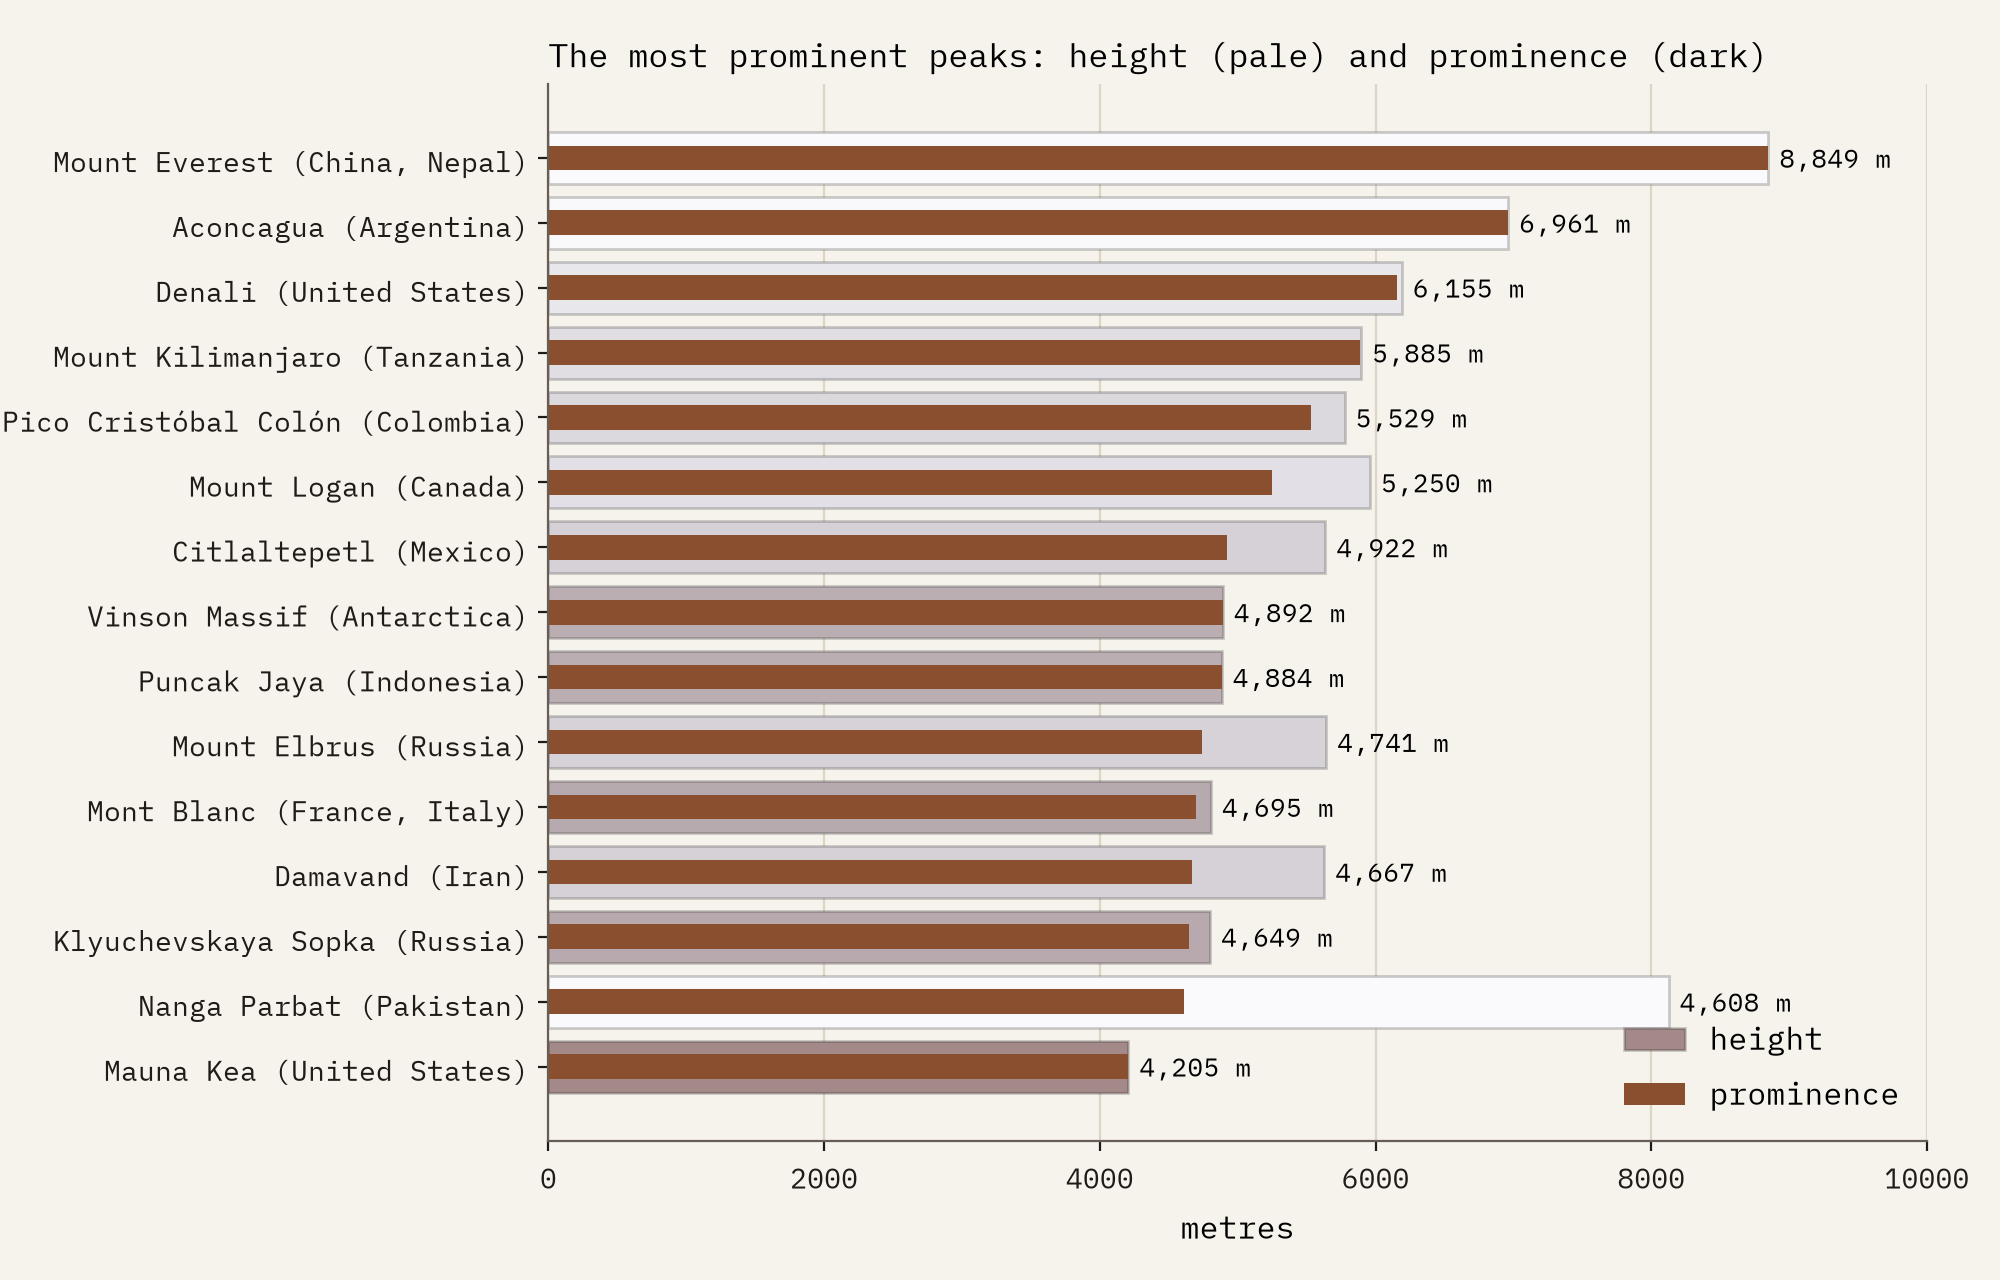
\includegraphics[width=.92\linewidth]{b_prominence.png}\caption{The fifteen most prominent peaks: height (pale) and prominence (dark). From English Wikipedia's list of peaks by prominence.}\label{fig:prom}\end{figure}

\subsection{Where people live}
The 4,325 cities kept hold 2.6 billion people by Wikidata's figures. Half of them live below 92 m. 10.3\% live above 1,000 m and 1.9\% above 2,000 m, against 26\% and 11\% of the land: above 2,000 m the land's share is 5.7 times the people's, or 3.4 times without Antarctica (Figure~\ref{fig:people}). 92 cities are above 2,000 m and 18 above 3,000 m. The highest city of a million or more is Quito (2,850 m); the most populous above 2,000 m are Mexico City, Bogotá and Addis Ababa (Figure~\ref{fig:cities}). La Paz is the highest capital (3,640 m), and Baku (-28 m) the lowest city of 100,000 or more.
\begin{figure}[tbp]\centering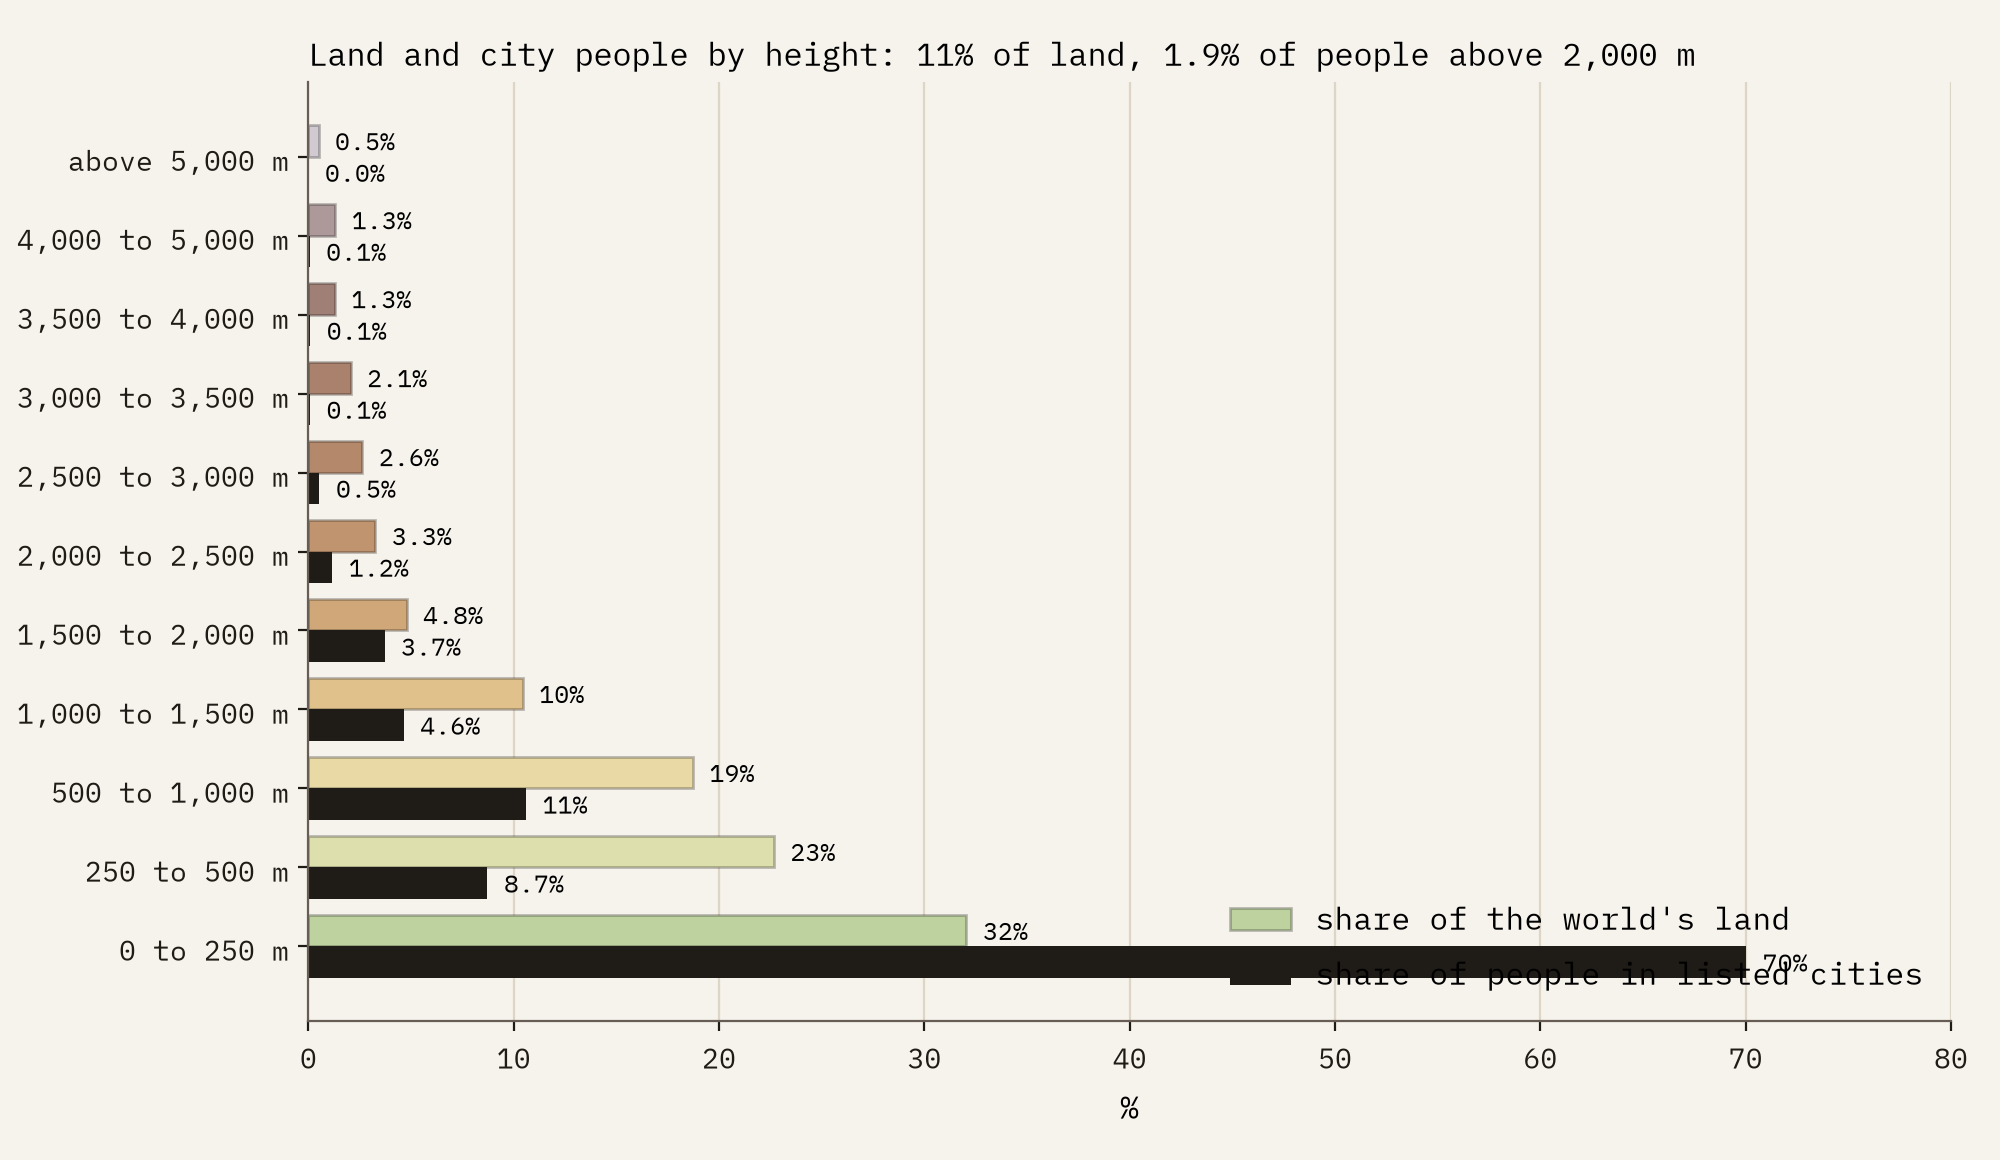
\includegraphics[width=.9\linewidth]{b_people_land.png}\caption{Share of the world's land and of the population of listed cities in each height band.}\label{fig:people}\end{figure}
\begin{figure}[tbp]\centering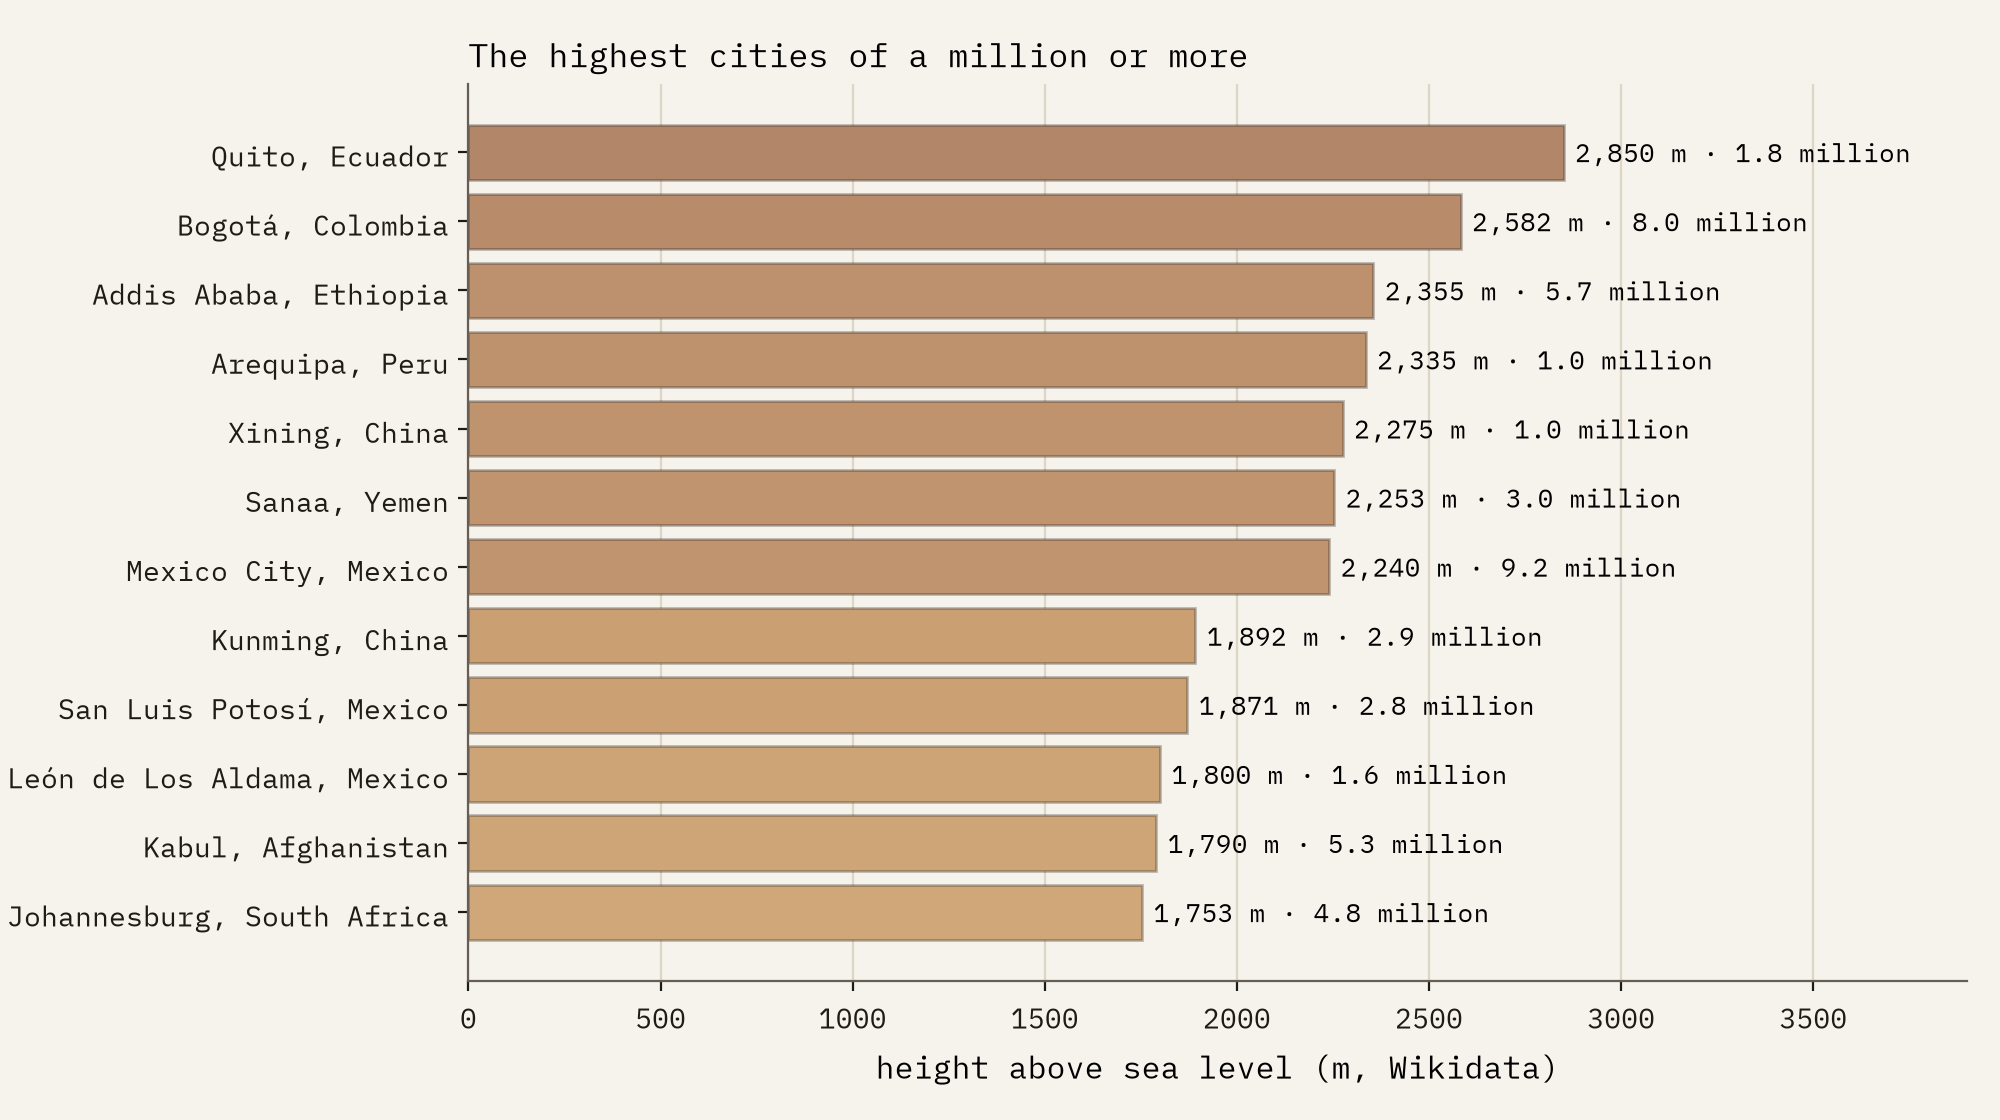
\includegraphics[width=.9\linewidth]{b_cities.png}\caption{The highest cities of a million or more (Wikidata heights and populations; Chinese cities by the urban population in Natural Earth).}\label{fig:cities}\end{figure}

\section{The interactive map}
The page loads the Terrarium tiles directly from Amazon's servers at whatever zoom the reader is viewing (0 to 14), decodes each pixel to a height in the browser and colours it with the same hypsometric palette as the figures. Hill shading uses Horn's gradient with light from the north-west and a vertical exaggeration that rises from 1 at zoom 11 to about 20 to 30 at the world view. Negative heights are drawn as land below sea level only inside Natural Earth's land with a trimmed coastline, and otherwise as sea floor. A reader can switch to shading only or to height steps with drawn class edges, grey out the land below any height (with the share of land and of city people above it), and click anywhere to read the height from a zoom 12 or finer tile. Peaks, cities by height, borders and place names are optional layers.

\section{Limitations}
The statistics come from a grid of about 10 km, so they understate peaks and narrow valleys, miss most small depressions and say little about countries smaller than about a hundred cells. Coastal cells are floored at sea level, which lowers coastal land slightly and hides coastal depressions. Lakes are removed using Natural Earth outlines, which do not match the tiles' lakes exactly; some lakes in the tiles carry floor depths. The terrain mosaic mixes sources of different ages and accuracies, and the ice surfaces of Antarctica and Greenland are those of their sources. The peak and city data come from Wikidata, whose heights and populations come from many sources and dates; despite the terrain checks some wrong heights will remain, especially low hills whose unit is wrong but whose value still looks plausible. Populations of Chinese prefecture-level cities include large rural areas. Sea level is a reference surface, not the level the sea actually reaches everywhere.

\section{Conclusion}
Open terrain tiles make it easy to describe the height of the whole planet and to let anyone explore it at any scale. The land is mostly low, with a quarter above 1,000 m and a tenth above 2,000 m, and much of that high land is ice; and people live far lower than the land lies, with fewer than one in fifty city dwellers in this data above 2,000 m.

\section*{Data and code availability}
The interactive map is at \url{https://maps.tristanhotham.com/world-terrain/}. Data and code are at \url{https://github.com/Tristan-Hotham/world-terrain} and archived with this paper at \url{https://doi.org/10.5281/zenodo.23848930}. Derived data are released under CC BY 4.0 (the table of prominent peaks under CC BY-SA 4.0, following Wikipedia) and code under the MIT licence. The terrain tiles themselves are not redistributed.

\section*{AI statement}
I wrote the text, with drafting and editing assistance from Claude (Anthropic), which also helped prepare the analysis code. I reviewed and checked all text and results.

\begin{thebibliography}{9}
\bibitem[Amante and Eakins(2009)]{etopo1} Amante, C. and Eakins, B.W. (2009) ETOPO1 1 arc-minute global relief model: procedures, data sources and analysis. NOAA Technical Memorandum NESDIS NGDC-24. National Geophysical Data Center, NOAA. doi:10.7289/V5C8276M
\bibitem[AWS(2026)]{terraintiles} Registry of Open Data on AWS (2026) Terrain Tiles. \url{https://registry.opendata.aws/terrain-tiles/}
\bibitem[Danielson and Gesch(2011)]{gmted} Danielson, J.J. and Gesch, D.B. (2011) Global multi-resolution terrain elevation data 2010 (GMTED2010). U.S. Geological Survey Open-File Report 2011-1073.
\bibitem[Farr et al.(2007)]{srtm} Farr, T.G. et al. (2007) The Shuttle Radar Topography Mission. \emph{Reviews of Geophysics}, 45, RG2004.
\bibitem[Mapzen(2017)]{joerd} Mapzen (2017) Joerd: data sources and attribution for the Terrain Tiles. \url{https://github.com/tilezen/joerd/blob/master/docs/attribution.md}
\bibitem[Natural Earth(2026)]{naturalearth} Natural Earth (2026) 1:10m cultural and physical vectors. Public domain. \url{https://www.naturalearthdata.com/}
\bibitem[Strahler(1952)]{strahler} Strahler, A.N. (1952) Hypsometric (area-altitude) analysis of erosional topography. \emph{Geological Society of America Bulletin}, 63(11), 1117 to 1142.
\bibitem[Vrandečić and Krötzsch(2014)]{wikidata} Vrandečić, D. and Krötzsch, M. (2014) Wikidata: a free collaborative knowledgebase. \emph{Communications of the ACM}, 57(10), 78 to 85.
\bibitem[Wikipedia(2026)]{wpprom} Wikipedia contributors (2026) List of mountain peaks by prominence. English Wikipedia, CC BY-SA 4.0. \url{https://en.wikipedia.org/wiki/List_of_mountain_peaks_by_prominence}
\end{thebibliography}
\end{document}
